\documentclass[12pt]{article}
\usepackage{graphicx} %LaTeX package to import graphics
\graphicspath{{images/}} %configuring the graphicx package
\usepackage[absolute]{textpos}
\setlength{\TPHorizModule}{1mm}
\setlength{\TPVertModule}{1mm}

\renewcommand*\familydefault{\sfdefault} %% Only if the base font of the document is to be sans serif
\usepackage[T1]{fontenc}

\usepackage[left=20.0mm, right=30.0mm, top=50mm, bottom=20mm, headheight=45mm,  footskip= 12mm, headsep=6mm, marginparsep=0mm]{geometry}

\usepackage{graphicx}
\usepackage{xcoffins,calc,xcolor} % added


\usepackage[many]{tcolorbox}


\usepackage{fancyhdr}
\usepackage{lastpage}

\usepackage[backend=biber, style=nature]{biblatex}
\addbibresource{library.bib}


\usepackage{tabularx}
\usepackage{fancybox}
\usepackage{fancyhdr}
\pagestyle{fancy}
\newlength{\hfwidth}
\addtolength{\hfwidth}{16pt}
\addtolength{\hfwidth}{2\fboxrule}
\renewcommand{\headrulewidth}{0pt}
\fancyhf{}
\def\imagetop#1{\vtop{\null\hbox{#1}}}
\def\imagetop#1{\raisebox{-\height+\baselineskip}{#1}}

\lfoot{\vspace{-45mm}
\begin{tabular}{l | l |l }
	\hline
	\phantom{c} & \phantom{b} & \phantom{a}\\
 \raisebox{-3mm}{
\includegraphics[width=40mm]{emcl.png}} & \raisebox{1mm}{\small{\begin{tabular}{l}
	Universität Heidelberg \\
	Interdisziplinäres Zentrum für Wissenschaftliches Rechnen \\
	Engineering Mathematics and Computing Lab (EMCL) \\
	Im Neuenheimer Feld 205, 69120 Heidelberg \\
	Tel.: +49 6221 54 14521 \\
	http://emcl.iwr.uni-heidelberg.de 
 \end{tabular}}} & \raisebox{1mm}{\small{\begin{tabular}{l} Erstellt: 19.12.2023 \\ \\ \\ \\ \\ Seite \thepage  \phantom{a}von \pageref{LastPage} \end{tabular}}}
\end{tabular}
}

\begin{document}
	%\pagestyle{fancy}
	%\fancyfoot{} % clear all footer fields
	%\fancyfoot[LO]{HAllo}
	\begin{textblock}{1000}(-10,0)
		
\includegraphics{heading.png}
	\end{textblock}
\noindent Bachelorarbeit
\section*{Continuous Modeling of Extracellular Matrix Invasion by \\ Tumor Growth}
\begin{tabular}{l l}
	KandidatIn: & Maximilian Bing\\
	Betreuer: & Prof. Dr. Vincent Heuveline \\
	AnsprechpartnerIn: & Valentin Schmid \\
	Zeitraum: & 01.01.2024 - 01.04.2024
\end{tabular}
\newline
\subsection*{Description}
Cancer cells can migrate from the primary tumor and degrade the surrounding tissue. Continuous mathematical models have been used several times in the past to better understand this process. In this context, the model is usually based on at least three key species, the tumor cells, the surrounding tissue or extracellular matrix (ECM) and the matrix degradative enzymes (MDE). Early descriptions of this model type can be found in the work of Anderson et al. \cite{anderson_continuous_1998,anderson_mathematical_2000} and Chaplain et al. \cite{anderson_continuous_1998,chaplain_mathematical_2006,chaplain_mathematical_2006-1,franssen_mathematical_2019}. The underlying model is described as follows. Let $c$, $e$ and $m$ be the tumor cell density, the ECM density and the MDE concentration respectively. Then, the governing equations are given by
\begin{align}
	\frac{\partial c}{\partial t} &= D_c \Delta c - \chi \nabla \cdot (c\nabla e) + \mu_1 c\left(1-\frac{c}{c_0}-\frac{e}{e_0}\right)\\
	\frac{\partial e}{\partial t} &= -\delta m e  + \mu_2 c\left(1-\frac{c}{c_0}-\frac{e}{e_0}\right)\\
	\frac{\partial m}{\partial t} &= D_m¸ \Delta c + \mu_3 c - \lambda m
\end{align}
with zero-flux boundary conditions 
\begin{align}
	n\cdot (-D_c \nabla c + c \chi\nabla f) &= 0 \\
	n \cdot (-D_m\nabla m ) &= 0
\end{align}
\newpage
\newgeometry{left=20.0mm, right=40.0mm, top=20mm, bottom=20mm, headheight=45mm,  footskip= 12mm, headsep=6mm, marginparsep=0mm}
\noindent Here, $D_c$ and $D_m$ are the diffusion coefficients, $\chi$ is the positive haptotactic coefficient, $\delta$ is a positive constant and $\mu_1$,$\mu_2$,$\mu_3$ and $\lambda$ are the production and decay constants. \newline 
The analysis of this models is mostly done in $1D$ in the literature and individual examples were done in 2D. However, preliminary reproductions of the model show that higher dimensions produce significantly different results, as can be seen in Figure \ref{fig:fig1}.
 \begin{figure}[!h]
 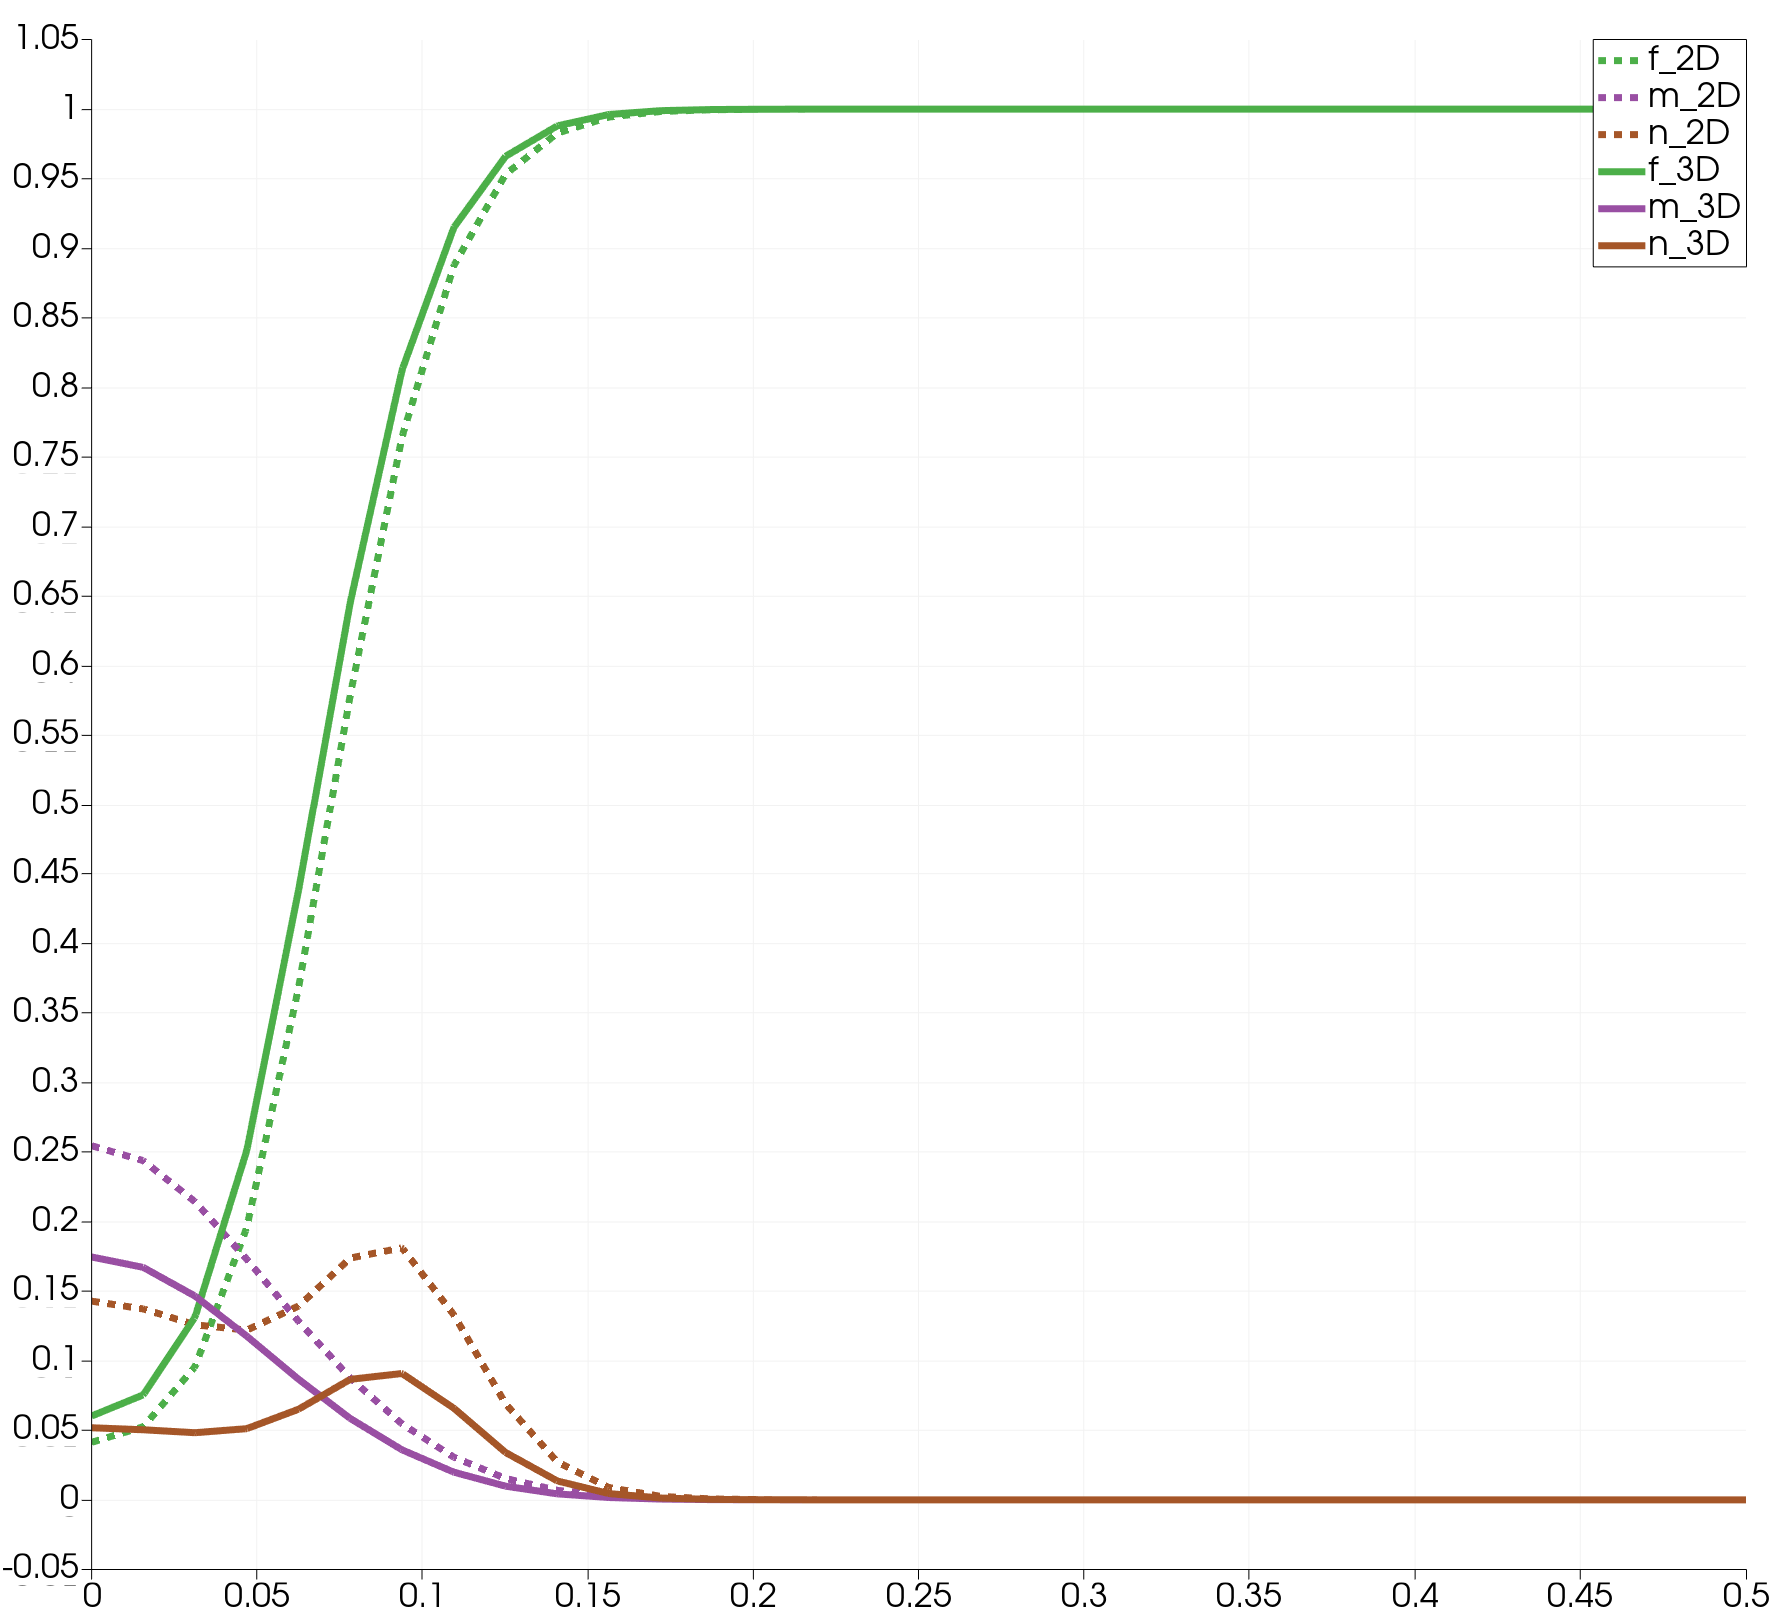
\includegraphics[width=0.45\textwidth]{anderson_tumor_invasion_model_2Dvs3Dtime0_7_thick.png}
 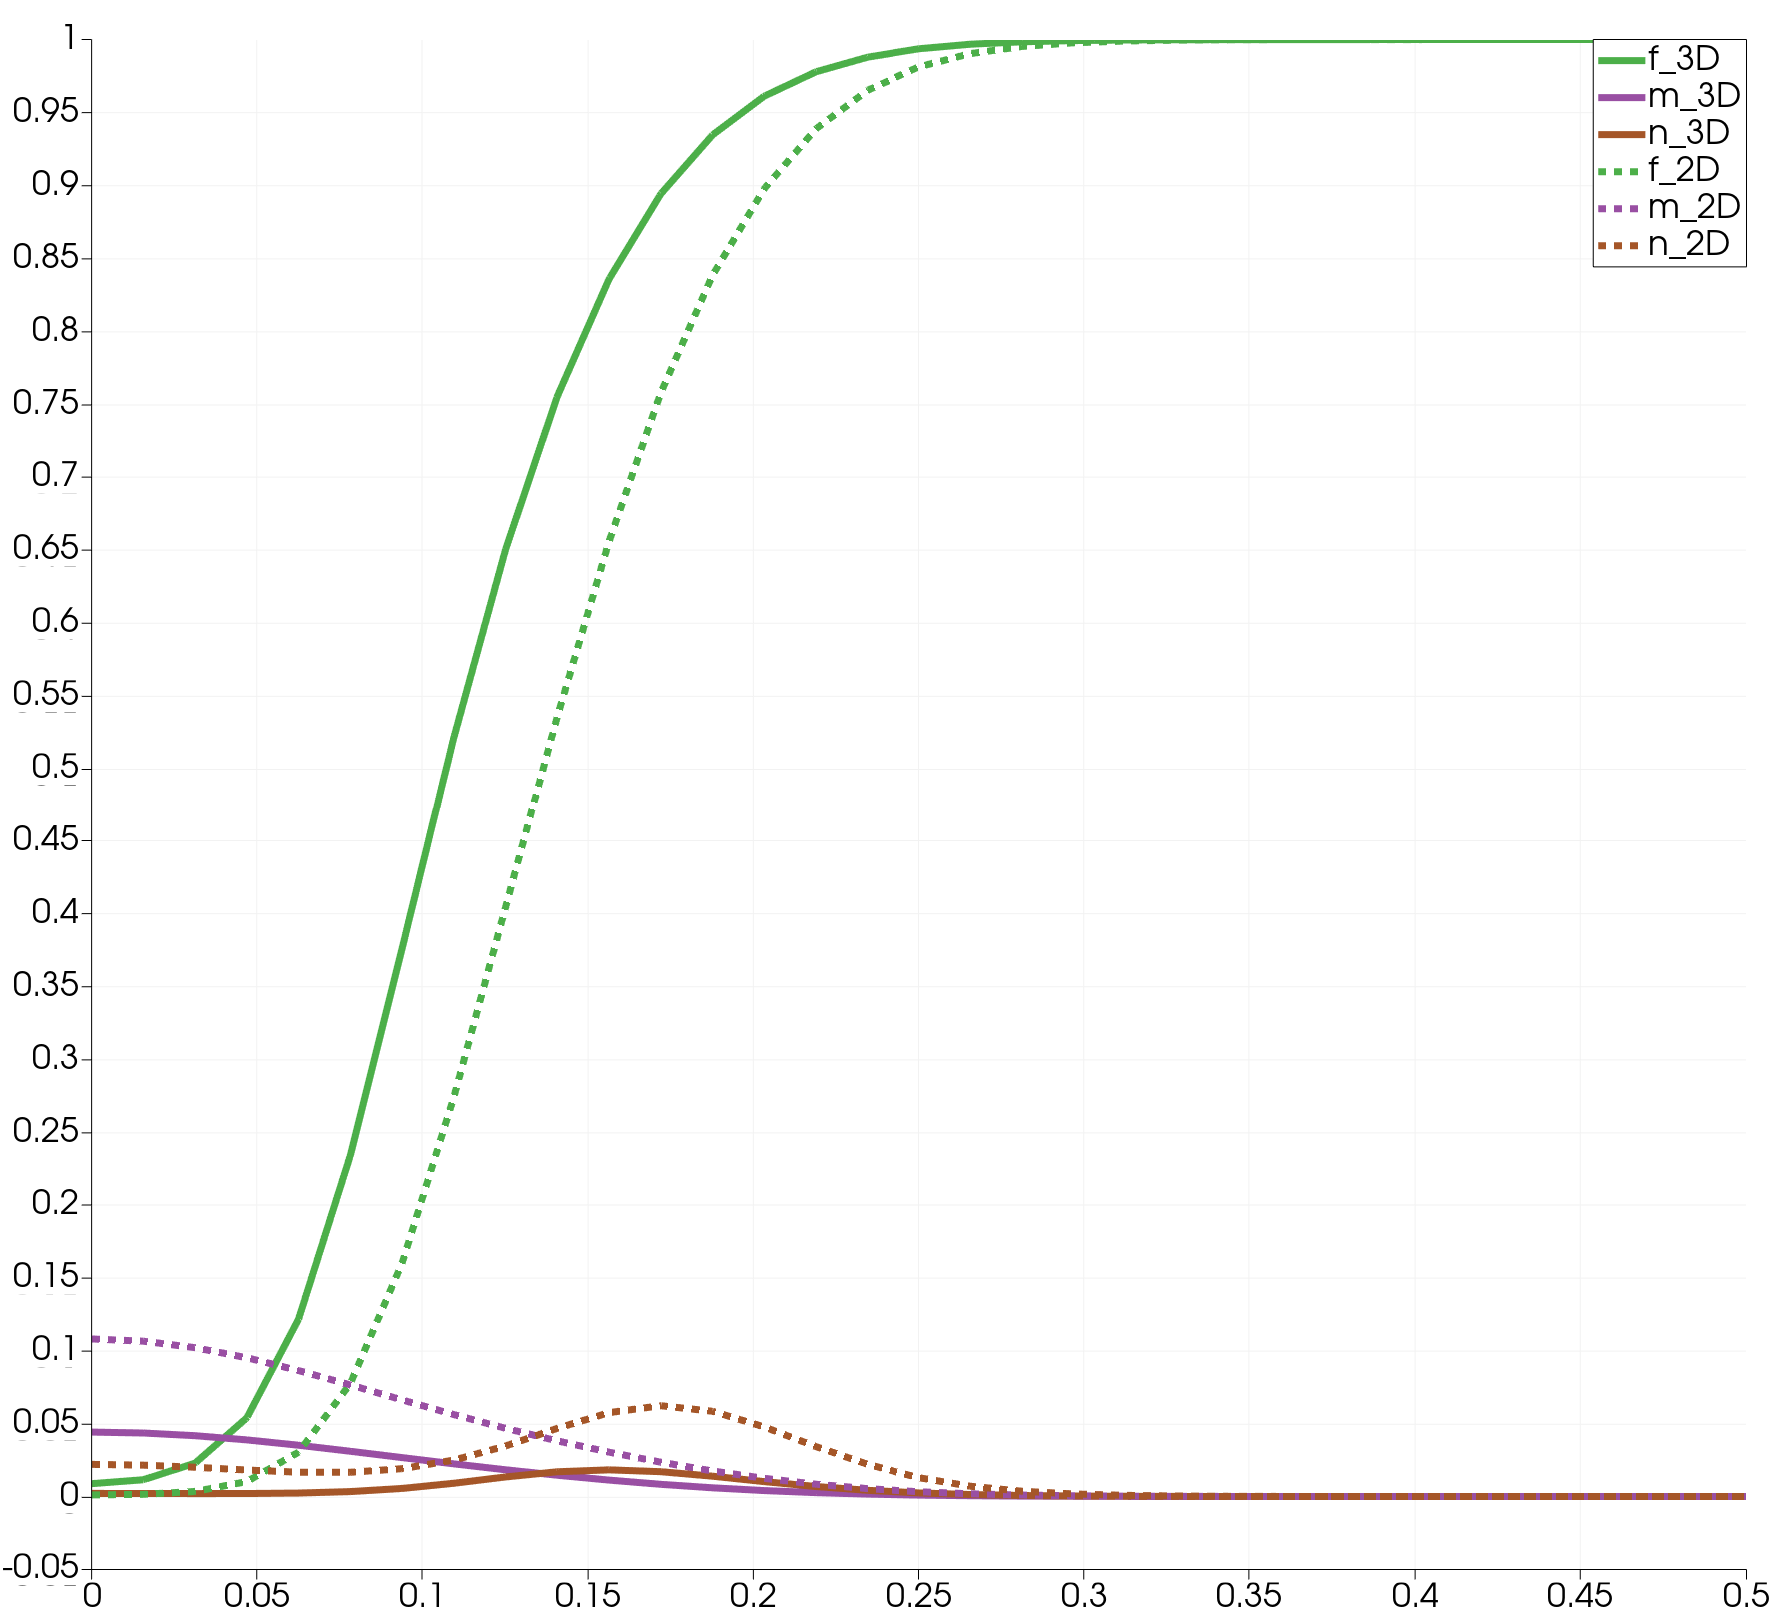
\includegraphics[width=0.45\textwidth]{anderson_tumor_invasion_model_2Dvs3D_time3_thick.png}
 \caption{Preliminary simulation results in 2D and 3D of the above described model at dimensionless time $t=0.7$ and $t=3$ and parameters $D_c=D_m=1e-3$, $\chi=5e-3$, $\delta=10$, $\mu_3=0.1$ and $\lambda=\mu_1=\mu_2 = 0$. }
 \label{fig:fig1}
\end{figure}
 The question therefore arises as to whether the parameters for this model need to be selected differently for simulations in 2D or 3D, or whether the results and analysis for the one dimensional case is incorrect. \newline
 Furthermore, the heterogeneous ECM structure has been addressed in the literature. However, the structure of the epithelial layer and the adjacent extracellular matrix is more organized in biological tissue than in the simulations shown in \cite{anderson_mathematical_2000} and \cite{chaplain_mathematical_2006-1}, for example. Therefore, simpler subdivisions of the geometry into ECM tissue could provide more meaningful results. \newline
 The aim of this work is to investigate the parameters and the model for higher dimensions on the one hand, and to consider a simple heterogeneity of the ECM structure on the other hand.
 \newpage
\printbibliography[title={Literatur}]
\newpage
\subsection*{Aufgabenstellung und Arbeitsplanung}
Mit einer Literaturrecherche wird zunächst gesammelt wie das oben angesprochene Modell bisher zum Einsatz kam. Zeitgleich kann mit der medizinischen Interpretation und Analyse des Modells begonnen werden. Im Anschluss daran soll vom Student eine kritische Evaluierung des Modells durchgeführt werden. Dabei soll unter anderem untersucht werden, ob die in der Literatur angegebenen Parameter auch für höhere Dimensionen sinnvoll sind. \newline
Währenddessen sollen die Ergebnisse anschaulich visualisiert und dokumentiert werden. Der Zeitrahmen für die jeweiligen Aufgaben kann in der folgenden Tabelle gefunden werden. 
\subsection*{Zeitplanung}
\begin{center}
\begin{tabular}{| c || c | c |c |c |c |c |c |c |c |c |c |c |c| c |}
  \hline
  Woche & 1 & 2 & 3 & 4 & 5 & 6 & 7 & 8 & 9 & 10 & 11 & 12 & 13 & 14 \\
  \hline
  \hline 
  Literaturrecherche & X & X & X  &  X & X  & X  & X  & & & & & & & \\
            \hline  
  Interpretation und Analyse & & X &  X & X  &X  &X  &X  &X  &X  & & & & & \\  
            \hline  
    Kritische Evaluierung & & & & & X  &X  &X  & X  &X  &X  &X  &X  & & \\  
              \hline  
      Visualisierung & & & & & & X &X  &X  &X  &X  &X  &X  & X  & \\  
                \hline  
        Dokumentation & & X& X& X& X& X& X& X& X& X & X& X&X &X \\  
                  \hline  
          Präsentation & & & & & & & & & & & & & X &X \\ 
          \hline  
\end{tabular}
\end{center}
\newpage
\subsection*{Besprechungen, Vortrag und Prüfungsordnung}
Zu Beginn, während und am Ende der studentischen Abschlussarbeit findet eine Besprechung des Kandidaten mit dem Betreuer statt. In einem zweiwöchigen Turnus berichtet der Kandidat dem Ansprechpartner den Stand der Arbeit und es werden die weiteren Schritte für die jeweils nächsten zwei Wochen geplant. In einem Vortrag im Bachelor-, bzw. Masterseminar wird die Arbeit abschliessend vorgestellt. Masterkandidaten stellen zu Beginn der Abschlussarbeit ihr Thema in einem Kurzvortrag der Arbeitsgruppe vor. Für die Erstellung und Abgabe der Arbeit sowie für den abschliessenden Vortrag gelten die Bestimmungen der jeweiligen Studienordnung, bzw. des jeweiligen Modulhandbuches.\newline 
\phantom{a}\newline
\phantom{a}\newline  
\vspace{30mm}
\begin{tabular}{| l | l | l | p{0.3\textwidth} |} 
	\hline 
	Funktion & Name & Datum & Unterschrift \\
	\hline 
	\hline 
	Kandidat & Maximilian Bing & & \begin{tabular}{c} \phantom{a} \\ \phantom{b}\end{tabular} \\
	\hline 
	Betreuer & Prof. Dr. Vincent Heuveline & & \begin{tabular}{c} \phantom{a} \\ \phantom{b}\end{tabular}\\
	\hline 
	Ansprechpartner &  Valentin Schmid& & \begin{tabular}{c} \phantom{a} \\ \phantom{b}\end{tabular}\\
	\hline 
\end{tabular}


\end{document}